
\begin{figure}[htbp]
\centering
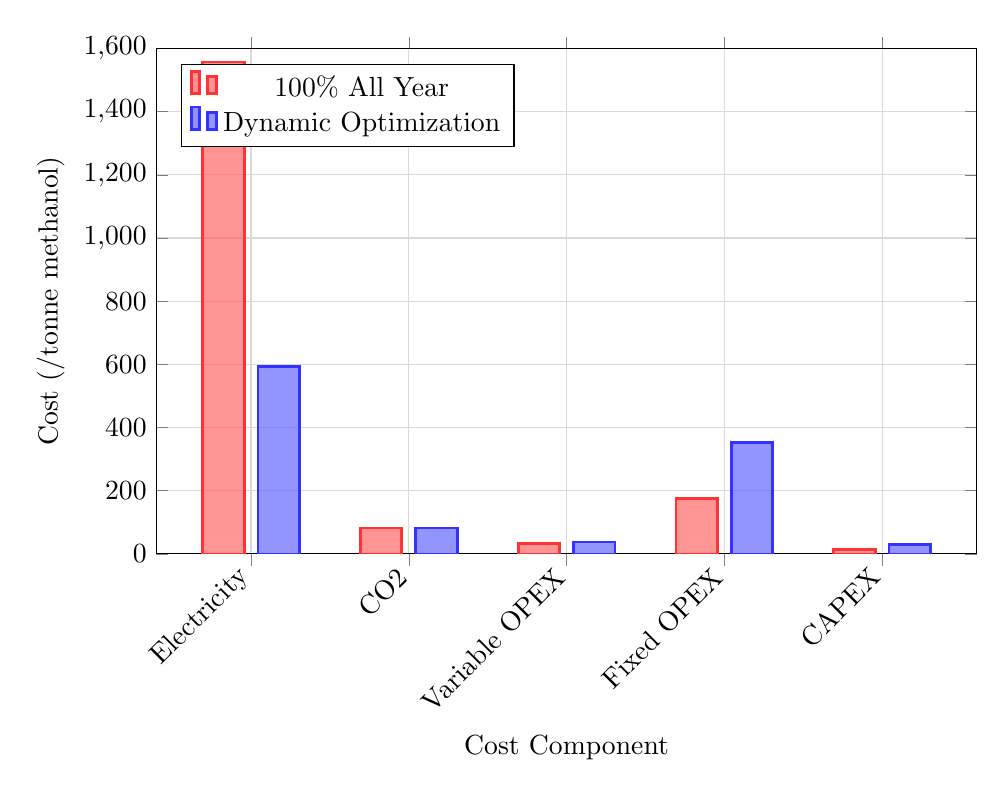
\begin{tikzpicture}
\begin{axis}[
    width=12cm,
    height=8cm,
    xlabel={Cost Component},
    ylabel={Cost (\euro/tonne methanol)},
    ymin=0,
    ymax=1600,
    xtick=data,
    symbolic x coords={Electricity,CO2,Variable OPEX,Fixed OPEX,CAPEX},
    legend pos=north west,
    grid=major,
    grid style={gray!30},
    bar width=15pt,
    ybar=5pt,
    enlarge x limits=0.15,
    x tick label style={rotate=45,anchor=east},
    every axis plot/.append style={
        fill opacity=0.7,
        draw opacity=1,
        line width=1pt
    }
]

% 2022 data (highest electricity prices) - 100% strategy
\addplot[
    fill=red!60,
    draw=red!80,
] coordinates {
    (Electricity,1557)
    (CO2,82)
    (Variable OPEX,32)
    (Fixed OPEX,176)
    (CAPEX,15)
};

% 2022 data - Dynamic strategy
\addplot[
    fill=blue!60,
    draw=blue!80,
] coordinates {
    (Electricity,593)
    (CO2,82)
    (Variable OPEX,38)
    (Fixed OPEX,352)
    (CAPEX,29)
};

\legend{100\% All Year, Dynamic Optimization}

\end{axis}
\end{tikzpicture}
\caption{Cost breakdown comparison for 2022 data (highest electricity price year)}
\label{fig:cost-breakdown}
\end{figure}
